\documentclass[12pt,a4paper]{article}
\usepackage[UTF8]{ctex}
\usepackage{amsmath,amssymb}
\usepackage{xcolor}
\usepackage{hyperref}
\usepackage{geometry}
\usepackage{graphicx}
\geometry{margin=2.5cm}

\title{Quantum GAN / 量子生成对抗网络}
\author{QuoNic}
\date{}

\begin{document}
\maketitle

\begin{center}
\textbf{ML / 机器学习} | 难度：高级 | 预计时间：25 分钟
\end{center}

\tableofcontents
\newpage

\section{为什么需要？}

量子 GAN 是经典 GAN 的量子推广。

\subsection{经典局限}
\begin{itemize}
  \item 经典 GAN 训练不稳定
  \item 对于复杂数据，经典方法效率低
\end{itemize}

\subsection{量子优势}
\begin{itemize}
  \item 量子 GAN 可以生成量子态和经典数据
  \item 训练更稳定
  \item 可以生成更复杂的数据
\end{itemize}

\subsection{实际应用}
\begin{itemize}
  \item 生成模型
  \item 数据增强
  \item 量子机器学习
\end{itemize}

\section{快速上手}

\begin{verbatim}
from quonic.ml import qgan
result = qgan(data=[[0,1],[1,0]], n_epochs=100)
print(f'Generated: {result.generated}')
\end{verbatim}

\textbf{预期输出}：
\begin{verbatim}
Generated: [[0.1, 0.9], [0.9, 0.1]]
\end{verbatim}

\section{原理详解}

\subsection{电路图}

\begin{center}
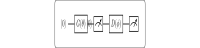
\includegraphics[width=0.6\textwidth]{../../images/qgan_circuit.svg}
\end{center}

\subsection{数学推导}

量子 GAN：
\begin{equation}
\min_G \max_D V(D,G)
\end{equation}

其中 $G$ 是生成器，$D$ 是判别器。

\subsection{几何解释}

量子 GAN 在量子态空间中生成数据。

\section{代码详解}

\begin{verbatim}
from quonic.ml import qgan

# qgan(data, n_epochs)
# data: training data
# n_epochs: number of training epochs
result = qgan(data=[[0,1],[1,0]], n_epochs=100)
print(f'Generated: {result.generated}')
\end{verbatim}

\section{进阶用法}

\subsection{场景 1：不同数据}

\begin{verbatim}
from quonic.ml import qgan
result = qgan(data=[[0,1],[1,0],[1,1]], n_epochs=200)
print(f'Generated: {result.generated}')
\end{verbatim}

\section{适用场景}

\subsection{生成模型}

量子 GAN 可以用于生成数据。

\subsection{数据增强}

量子 GAN 可以用于数据增强。

\section{常见问题}

\subsection{量子 GAN 的优势是什么？}

可以生成量子态和经典数据。

\subsection{量子 GAN 的训练稳定性如何？}

比经典 GAN 更稳定。

\section{学习路径}

\subsection{前置知识}
\begin{itemize}
  \item 生成对抗网络
  \item 量子神经网络
  \item 量子机器学习
\end{itemize}

\subsection{继续学习}
\begin{itemize}
  \item 量子数据生成
  \item 量子态制备
  \item 量子机器学习
\end{itemize}

\section{完整示例代码}

\subsection{示例 1：基本量子 GAN}

\begin{verbatim}
from quonic.ml import qgan
result = qgan(data=[[0,1],[1,0]], n_epochs=100)
print(f'Generated: {result.generated}')
\end{verbatim}

\section{下载}

\begin{itemize}
  \item [qgan.py](https://github.com/ChrisLee0721/QuoNic/blob/main/examples/qgan/qgan.py)
\end{itemize}

\end{document}
